\documentclass[letterpaper, 8pt]{extarticle}
\usepackage{amssymb,amsmath,amsthm,amsfonts}
\usepackage{multicol,multirow}
\usepackage{calc}
\usepackage{ifthen}
\usepackage[landscape]{geometry}
\usepackage[colorlinks=true,citecolor=blue,linkcolor=blue]{hyperref}
\usepackage{booktabs}
\usepackage{ulem}
\usepackage{enumitem}
\usepackage{tabulary}
\usepackage{graphicx}
\usepackage{siunitx}
\usepackage{tikz}
\usepackage{derivative}
\usepackage{svg}
\usepackage{listings}
\usepackage{color}
\usepackage{soul}
\usepackage{clrscode3e}


\ifthenelse{\lengthtest { \paperwidth = 11in}}
    { \geometry{top=.25in,left=.25in,right=.25in,bottom=.25in} }
	{\ifthenelse{ \lengthtest{ \paperwidth = 297mm}}
		{\geometry{top=1cm,left=1cm,right=1cm,bottom=1cm} }
		{\geometry{top=1cm,left=1cm,right=1cm,bottom=1cm} }
	}

\newenvironment{Figure}
  {\par\medskip\noindent\minipage}
  {\endminipage\par\medskip}

\pagestyle{empty}
\makeatletter
\renewcommand{\section}{\@startsection{section}{1}{0mm}%
                                {-1ex plus -.5ex minus -.2ex}%
                                {0.5ex plus .2ex}%x
                                {\normalfont\normalsize\bfseries}}
\renewcommand{\subsection}{\@startsection{subsection}{2}{0mm}%
                                {-1explus -.5ex minus -.2ex}%
                                {0.5ex plus .2ex}%
                                {\normalfont\small\bfseries}}
\renewcommand{\subsubsection}{\@startsection{subsubsection}{3}{0mm}%
                                {-1ex plus -.5ex minus -.2ex}%
                                {1ex plus .2ex}%
                                {\normalfont\tiny\bfseries}}
\makeatother
\setcounter{secnumdepth}{0}
\setlength{\parindent}{0pt}
\setlength{\parskip}{0pt plus 0.5ex}
% -----------------------------------------------------------------------
% \tymin=37pt
% \tymax=\maxdimen

% Custom siunitx defs
\DeclareSIUnit\noop{\relax}

\NewDocumentCommand\prefixvalue{m}{%
\qty[prefix-mode=extract-exponent,print-unity-mantissa=false]{1}{#1\noop}
}

% Shorthand definitions
% \newcommand{\To}{\Rightarrow}

% condense itemize & enumerate
\let\olditemize=\itemize \let\endolditemize=\enditemize \renewenvironment{itemize}{\olditemize \itemsep0em}{\endolditemize}
\let\oldenumerate=\enumerate \let\endoldenumerate=\endenumerate \renewenvironment{enumerate}{\oldenumerate \itemsep0em}{\endoldenumerate}

\title{2C03}

\begin{document}

\raggedright
\tiny

\begin{center}
  {\textbf{2C03}} \\
\end{center}
\begin{multicols*}{4}
  \setlength{\premulticols}{1pt}
  \setlength{\postmulticols}{1pt}
  \setlength{\multicolsep}{1pt}
  \setlength{\columnsep}{2pt}

  \section{Algorithms}
  
  \section{Basic DSes}
  Array vs LL

  \textbf{Arrays:}
  Static data sets, ones where fast index-based access is needed,
  Slow expansion, insertion, deletion.
  \textbf{LLs:}
  Dynamic data sets,
  insertion \& deletion more important than random access.


  % REVIEW: Probably don't need LLs,
  % pretty easy to reason through
  % REVIEW: Are there any other basic data structures that need more detail? 
  \subsection{Linked Lists}
  \begin{lstlisting}[language=Java, breaklines=true, postbreak=\mbox{\textcolor{red}{$\hookrightarrow$}\space}]
class Node {
    Item item;
    Node next;
    Node prev; // for DLL
}
    \end{lstlisting}
  \subsubsection{Operations}
  \begin{tabular}[!ht]{@{}ll@{}} \toprule
    Search           & O(N) \\
    Prepend / Append & O(1) \\
    Delete           & O(N) \\
    \bottomrule
  \end{tabular}

  \section{Runtime Analysis}
  \begin{tabular}[!ht]{@{}lc@{}} \toprule
    constant     & 1          \\
    logarithmic  & $\log N$   \\
    linear       & $N$        \\
    linearithmic & $N \log N$ \\
    quadratic    & $N^2$      \\
    cubic        & $N^3$      \\
    exponential  & $2^N$      \\
    \bottomrule
  \end{tabular}

  % REVIEW: Make sure there are no errors, and that there are no important algos missed
  \subsection{Sorting Algorithm Info}
  \begin{tabular}[!ht]{@{}llll@{}} \toprule
    Algorithm      & $O(N)$        & $\Omega(N)$        & $\Theta(N)$        \\
    \midrule
    Selection Sort & $O(N^2)$      & $\Omega(N^2)$      & $\Theta(N^2)$      \\
    Insertion Sort & $O(N^2)$      & $\Omega(N)$        & $\Theta(N^2)$      \\
    Shellsort      & $\leq O(N^2)$ & $\Omega(N \log N$) & $\Theta(N \log N)$ \\
    Mergesort      & $O(N \lg N)$  & $\Omega(N \lg N)$  & $\Theta(N \lg N)$  \\
    Quicksort      & $O(N^2)$      & $\Omega(N \lg N)$  & $\Theta(N \lg N)$  \\
    Heapsort       & $O(N \log N)$ & $\Omega(N \log N)$ & $\Theta(N \log N)$ \\
    \bottomrule
  \end{tabular}
  \begin{tabulary}{\linewidth}{@{}LllL@{}} \toprule
    Algorithm       & Stbl? & In-Place? & Space \\
    \midrule
    Selection Sort  & N     & Y         & O(1) \\
    *Insertion Sort & Y     & Y         & O(1) \\
    Shellsort       & N     & Y         & O(1) \\
    **Quicksort     & N     & Y         & O($\log N$) \\
    Mergesort       & Y     & N         & O($N$) \\
    Heapsort        & N     & Y         & O(1) \\
    \bottomrule
  \end{tabulary} \\
  * depends on order of items \\
  ** probabilistic guarantee

  \subsection{Tilde Approximation}
  $\lim_{n \to \infty} \frac{~f(n)}{f(n)} = 1$
  TL;DR drop everything but the most significant factor in terms of $n$.

  \subsection{Order of Growth}
  Just drop the constant from the tilde approximation

  % REVIEW: Look back through this explanation
  \subsection{Proving}
  For any pair of constants, $c, n_0$, consider $n = X[c \cdot n_0]$,
  where $X$ is another arbitrarily chosen constant.

  If a pair can be found that satisfies these constants, then list them.
  If a pair cannot be found, prove that there exists a contradiction.

  \subsection{Big-O}
  Upper limit, function must be $\leq O(n)$

  $\lim_{n \to \infty} \frac{f(n)}{g(n)} \neq \infty$

  \subsection{Big-\texorpdfstring{$\Omega$}{Omega}}
  Lower limit, function must be $\geq \Omega(n)$

  $\lim_{n \to \infty} \frac{f(n)}{g(n)} \neq 0$

  \subsection{Big-\texorpdfstring{$\Theta$}{Theta}}
  Must satisfy both Big-O and Big-$\Omega$.

  $\lim_{n \to \infty} \frac{f(n)}{g(n)} \not\in \{0, \infty\}$

  % REVIEW: Are there any other algs 
  % that we need to document for memory complexity?
  \subsection{Memory Complexity}
  \textbf{In-place algorithms:} $N + O(\log N)$
  \textbf{Mergesort:}
  Original input array: $N$.
  Aux array for merging: $N$.
  Local variables: $Const$.
  Function call stack: $\log N$.
  Total: $2N + O(\log N)$.

  \subsection{Recurrence Relations}

  % yea, basically this algorithm splits the tree into two sides with a 1-9 ratio, 
  % the sum of each layer is always n, so the time complexity is 
  % $n * \log{\text{depth of the tree}} n$. 
  % The 9/10 side will run out of nodes slower, 
  % so it's $n \log{10/9}$ since it takes 10/9 steps to have only one node left 
  % because $10/9 * 9/10 = 1$. \\
  % - youcef

  \textbf{Deriving from a Tree:}
  Represent the recurrence equation as a binary tree,
  where each layer is one layer deeper in the recursion.
  Eg if the equation is $T(N) = T(N/2) + T(N/2)$,
  there will be 2 branches on the second layer, each as $T(N/2)$,
  4 branches on the third layer, each as $T(N/4)$, and so on.
  If it's a binary tree, with $x$ layers,
  it will have a time complexity of $n \log x$.
  \hl{If you're seeing this, please contribute!}
  % FIXME: ADD THIS

  \section{Union-Find}
  WARNING: !CODE DOES NOT IMPLEMENT COUNT! \\
  In a network of nodes, mutually connected are called components. Union find has the following api:
  \begin{itemize}
      \item \textbf{Connected}: takes two nodes, return true if nodes are in the same component
      \item \textbf{Union}: if not connected, connects two nodes
      \item \textbf{Find}: takes node id, returns the component the node is in
      \item \textbf{Count}: return number of components
  \end{itemize}
  Rather than classes or data structures, we can optimize the api by using a structure that allows us to just perform our operations.
  Key learnings:
  \begin{itemize}
      \item Generally, either optimize for adding data into Data Structure,
            or optimize for processing the Data Structure for desired results.

      \item
  \end{itemize}

  \subsection{Time Complexity}
  \begin{tabular}[!ht]{@{}llll@{}} \toprule
      Algo           & Q-F    & Q-U    & WQ-U       \\
      \midrule
      Initialization & $O(N)$ & $O(N)$ & $O(N)$     \\
      Find           & $O(1)$ & $O(N)$ & $O(lg(N))$ \\
      Connected      & $O(1)$ & $O(N)$ & $O(lg(N))$ \\
      Union          & $O(N)$ & $O(N)$ & $O(lg(N))$ \\
      \bottomrule
  \end{tabular}

  \subsection{Quick-Find}
  For Quick-Find, instead of associating nodes with connections, we associate them with components. We can represent the graph with an array. Indices of the array act as the node ids and the values act as the component ids. We also need a count variable.
  \subsubsection{Initialization}
  Create array of length N, iterate through it and initialize each element to the value of it's index
  \subsubsection{Union}
  Takes two indices, p and q. Iterate through array and change every occurrence of arr[p] to arr[q], or vice versa.
  \subsubsection{Find}
  Takes an index, returns value at index
  \subsubsection{Connected}
  Takes two indices, p and q, returns if arr[p] = arr[q]\\
  \begin{lstlisting}[language=Java, breaklines=true, postbreak=\mbox{\textcolor{red}{$\hookrightarrow$}\space}]
public class QuickFind {
  private int[] id;
  
  public QuickFind(int N) {
      count = N;
      id = new int[N];
      for(int i = 0; i < N; i++)
          id[i] = i;
  }
  public int find(int p) {
      return id[p];
  }
  public void union(int p, int q) {
      int pid = id[p];
      int qid = id[q];
      for(int i = 0; i < id.length;i++)
          if(id[i] == pid) id[i] = qid;
  }
  public boolean connected(int p, int q) {
      return id[p] == id[q];
  }
}
  \end{lstlisting}
  
  \subsection{Quick-Union}
  Quick-Union also uses an array to represent the graph, but is interpreted differently. The indices still represent node ids, but the values now also represent node ids. The values point to the node's parent node. This representation forms a tree structure, where the root node points to itself. This means we can use the id of root nodes as component ids.
  \subsubsection{Initialization}
  Create array of length N, iterate through it and initialize each element to the value of it's index
  \subsubsection{Union}
  Takes an indices p and q, finds the root nodes. If they are not equal, make one point to the other.
  \subsubsection{Find}
  Takes an index i, finds arr[i] until the root node. Returns the root node id.
  \subsubsection{Connected}
  Takes an indices p and q, finds the root nodes. Returns true if they are equal.
  \begin{lstlisting}[language=Java, breaklines=true, postbreak=\mbox{\textcolor{red}{$\hookrightarrow$}\space}]
public class QuickUnion {
  private int[] id;
  
  public QuickUnion(int N) {
      id = new int[N];
      for(int i = 0; i < N; i++)
          id[i] = i;
  }
  public int find(int i) {
      while (i != id[i]) {
          i = id[i]
      }
      return i;
  }
  public void union(int p, int q) {
      int i = find(p);
      int j = find(q);
      id[i] = j;
  }
  public boolean connected(int p, int q) {
      return find(p) == find(q);
  }
}
  \end{lstlisting}
  
  \subsection{Weighted Quick-Union}
  To optimize Quick-Union, we try to create the flattest trees possible. We need another array to count the number of nodes rooted at an index. Union now links the root of the smaller tree to the root of the larger tree. This can be further optimized with path compression, which can be tacked on to find. To do this, we change each node to point at it's grandparent.
  \begin{lstlisting}[language=Java, breaklines=true, postbreak=\mbox{\textcolor{red}{$\hookrightarrow$}\space}]
public class WeightedQuickUnionWithPC {
  private int[] id;
  private int[] sz;
  
  public void union(int p, int q) {
      int i = find(p);
      int j = find(q);
      id[i] = j;
      if (sz[i] < sz[j])   { id[i] = j; sz[j] += sz[i] }
      else (sz[i] < sz[j]) { id[j] = i; sz[i] += sz[j] }
  }
  public int find(int p) {
      while (i != id[i]) {
          id[i] = id[id[i]];
          i = id[i];
      }
      return i;
  }
  \end{lstlisting}

  % FIXME: For *all* the sorts, add pros and cons if possible!
  \section{Bad Sorts}
  \subsection{Selection Sort}
  Build up a sorted section of array, by
  \begin{enumerate}
    \item Find min element
    \item Swap min \& first element
    \item Examine array, skipping first element.
  \end{enumerate}
  $\Theta(N^2)$
  \subsection{Insertion Sort}
  Start from 2 elements, build up sorted subarray,
  "inserting" a new element each iteration by swapping
  until it is in the right position.
  The number of operations it takes to sort an array
  depends on the degree of disorder (how unsorted the array is).
  This makes it an adaptive algorithm.
  \begin{center}
    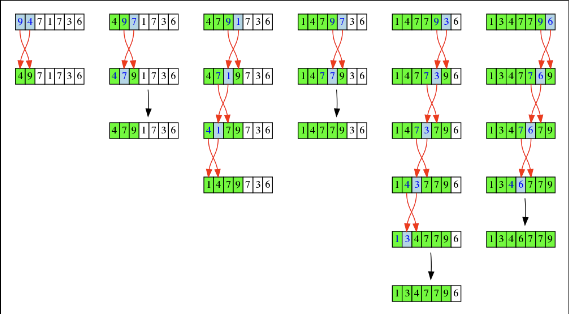
\includegraphics[width=\linewidth]{insertion-sort.png}
  \end{center}

  $\Omega(N), O(n^2)$
  \subsection{Shellsort}
  Pick every $n$ elements and put them in a subarray,
  sort the subarrays using insertion sort, and put the elements back. Then reduce the gap from $n$.
  Repeat the process till $n$ is 1.
  (If you only use indicies you don't need to make a new array.)
  \begin{center}
    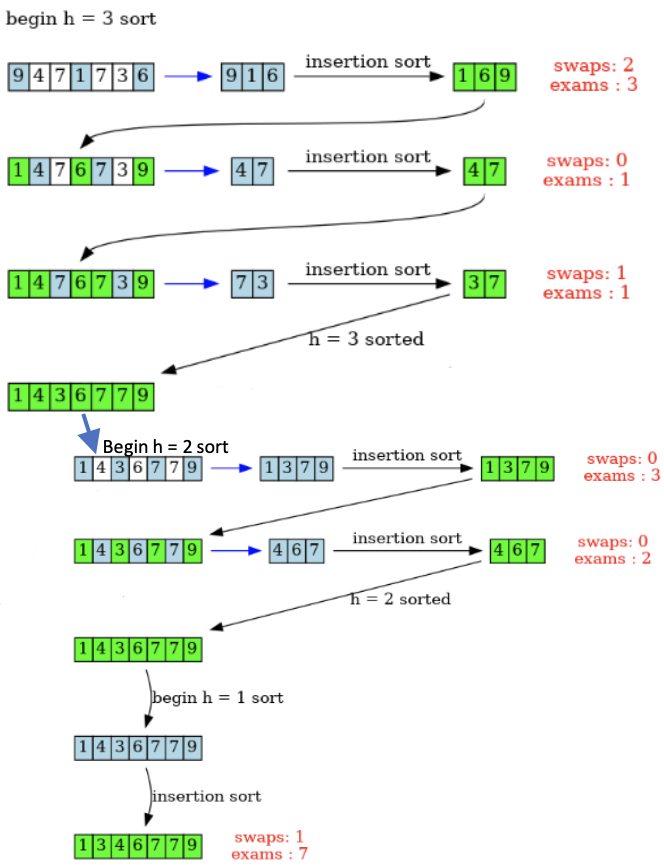
\includegraphics[width=\linewidth]{shellsort.png}
  \end{center}
  \begin{lstlisting}[language=Java, breaklines=true, postbreak=\mbox{\textcolor{red}{$\hookrightarrow$}\space}]
public class Shell {
  public static void sort(Comparable[] a) {
    int N = a.length;
    int h = 1;
    while (h < N/3) h = 3 * h + 1;
    while (h >= 1) {
      for (int i = h; i < N; i++) {
        for (int j = i; j >= h && less(a[j], a[j-h]); j -= h)
          exch(a, j, j-h);
      }
      h = h / 3;
    }
  }
}
  \end{lstlisting}
  % FIXME: Add time complexity

  \section{Good Sorts}
  \subsection{Mergesort}
  Divide array in half recursively, until it is down to 1 element.
  Merge array together,
  making sure each side is sorted as it is merged together.

  \textbf{Time Complexity:} $O(n \log n)$ \\
  \textbf{Memory Complexity:} $O(N)$

  \subsubsection{Bottom-up}
  % code from slides
  \begin{lstlisting}[language=Java, breaklines=true, postbreak=\mbox{\textcolor{red}{$\hookrightarrow$}\space}]
private static void merge(Comparable[] a, Comparable[] aux, int lo, int mid, int hi) {
  // copy
  for (int k = lo; k <= hi; k++)
    aux[k] = a[k];
  // merge
  int i = lo, j = mid + 1;
  for (knt i = lo; k <= hi; k++) {
    if (i > mid) 
      a[k] = aux[j++];
    else if
      (j > hi) a[k] = aux[i++];
    else if
      (less(aux[j], aux[i])) a[k] = aux[j++];
    else
      a[k] = aux(i++);
  }
}

private static void sort(Comparable[] a, Comparable[] aux, int lo, int hi) {
  if (hi <= lo) return;
  int mid = lo + (hi - lo) / 2;
  sort(a, aux, lo, mid);
  sort(a, aux, mid+1, hi);
  merge(a, aux, lo, mid, hi);
}

public static void sort(Comparable[] a) {
  Comparable[] aux = new Comparable[a.length];
  sort(a, aux, 0, a.length - 1);
}
    \end{lstlisting}

  \subsubsection{Top-down}
  % STUB: FINISH THIS

  \subsection{Quicksort}
  \hl{If you're seeing this, please contribute!}
  % FIXME: ADD THIS

  \section{Priority Queues}
  Supports insertion and removing/popping the priority (largest or smallest) item.

  Implementations:
  \begin{list}{}{}
    \item Sorted Array - O(n) insert, O(1) pop
    \item Unsorted Array - O(1) insert, O(n) pop
    \item Binary Heap - O(log n) insert and sort
  \end{list}

  \section{Binary Heaps \& Heapsort}
  A max binary heap is a complete binary tree where the keys are in the nodes and each parent's key $\geq$ each child's key. This requirement is called the max heap property.
  \\
  Binary Heaps:
  \begin{itemize}
    \item Can be represented as array or tree/nodes.
    \item Insertion: We insert at the end of the array, then "swim up" the value.
    \item Swimming up - exchange a given node with it's parent until the binary max property is fulfilled.
    \item Popping - swap the first node (the max) with the last node, remove it, then "sink" the first node.
    \item Sinking - exchange a given node with the max of it's children until the binary max property is fulfilled.
  \end{itemize}

  Heapsort relies on the binary heap data structure to sort data. Once a max heap has been constructed, you can perform a single for loop and call $RemoveMax$ to build a sorted array (thus linearizing the heap).

  \section{Binary Trees}
  \textbf{Binary Tree:} A tree where each internal node has at most two children.
  \textbf{Full Binary Tree:} A binary tree where each internal node has exactly two children.
  \textbf{Complete Binary Tree:} A complete binary tree is which every level, 
  except possibly the last, is completely filled, and all nodes are as far left as possible.
  $L = N - 1$, where $L$ is the number of the internal node in the tree,
  and $N$ is the number of leaves.

  $N = 2^h$, where $h$ is the height of the tree and $N$ is the number of nodes in the tree.
  To go the other way around, $\log_2(N) = h$.

  \section{Pseudocode}
  \begin{codebox}
  \Procname{$\proc{Insertion-Sort}(A)$}
  \li \For $j \gets 2$ \To $\attrib{A}{length}$
  \li   \Do
          $\id{key} \gets A[j]$
  \li     \Comment Insert $A[j]$ into the sorted sequence
            $A[1 \twodots j-1]$.
  \li     $i \gets j-1$
  \li     \While $i > 0$ and $A[i] > \id{key}$
  \li       \Do
              $A[i+1] \gets A[i]$
  \li         $i \gets i-1$
            \End
  \li     $A[i+1] \gets \id{key}$
        \End
  \end{codebox}
  Reminders:
  \begin{itemize}
    \item Attributes can be accessed via \verb|x.prev|.
    \item Class functions \textbf{do not exist in pseudocode}.
    Instead of calling \verb|x.sort()|, call \verb|sort(x)|.
    \item Use \verb|NIL| instead of \verb|null|.
    \item State assumptions like passing by value or passing by reference
    in the pseudocode.
    \item Use \verb|error| for throwing an error, but what happens is not specified.
  \end{itemize}

\end{multicols*}

\end{document}